\section{Personalization of Cardiac Biomechanics}


In order to make use of models 


\subsection{Data aquistition}

Since the discovery of X-ray in 1895, medical imaging has played a central
role in diagnosis, treatment planning and follow-up. Without the huge
advancements in medical imaging the last decades, computational models
would not have been as important and promising as it has become.

The interaction between cardiac images and cardiac models are important.


Still, one of the major bottlenecks in terms of personalized
computaional models is the quality of data (and representations of
model). There is a big issue in
reproducebility, because of noisy data, and operator depedent
measurements.

Today there are three main non-invasive imaging techniques used in
cardiology which is echocardiography (ECHO), magnetic
resonance imaging (MRI) and computed tomography (CT), and all of them
are used for aquiring data used in computaional modeling. Each
modality offers advantages and disadvatages over the other, and we
will make a short summary of pros and cons for each modelity below.

\subsubsection{CT}
Computed tomography is reconginzed as the 

\subsubsection{ECHO}

\subsubsection{MRI}






For example, MRI provides
high quality images, uses zero radiation, but is exspensive and lacks
temporal resolution. CT can more accuratley reconstruct the 3D image
in contrast to MRI, in which 2D slices needs to be glued together to
form a 3D surface. However, CT exposes the patient to radiation which
increases the chance of developing cancer. Finally echocardiography is
easy to use, cheap, harmless, and  has good temporal resolution, but
is clearly inferior when it comes to image quality.

The main modality used in this thesis is 4D echocardiography, and we
will therefore focus on data aquired using this modality.
With 4D we mean three spatial and one temporal dimesion.
In order to aquire a 3D volume image using ultrasound, the speed of sound in
human tissue (which is approxmately 1540 m/s) put some limitations on
the image quality verus the frame-rate \cite{rabben2010technical}.
Consequently, a 3D ultracound image is formed by stiching together $N$
disjoint subvolumes aquired during $N$ cardiac cycles ($N$ typicall
between 2 and 8)\cite{brekke2007volume}.

The images are later processed using some image segmentation tool.
One such tool is EchoPac which is used for analysing images for GE
Vingmed. The 4D Auto LVQ tool in EchoPac, is a tool for processing 3D
echo images, and traces of volume, triangulated surfaces and 3D strain
traces together with a structured mesh of the AHA segments for each
time point, can be exported to and HDF format and later used for mesh generation. 






\subsection{Geometry and microstructure}


\subsubsection{Mesh generation}
In this section we will explain how to generate a left ventricular
mesh based on segmented surfaces coming from 4D echocardiography.
Figure \ref{fig:echopac_output} shows an example of how the exported data
from the image semgentation tool looks like. For each time point we
can extract triangulated surfaces of the endocardium and epicardium
which can be seen in Figure \ref{fig:echopac_out_surf}. Together with
these surfaces we are also given a so called strain mesh (Figure
\ref{fig:echopac_out_strain_mesh}) located approximately in the
midwall, which defines the approximate location of the AHA-segments
\cite{cerqueira2002standardized}, and can be used to orient the mesh. 


\begin{figure}[htbp]
  \centering
  \begin{subfigure}[t]{0.45\textwidth}
    \includegraphics[width=\textwidth]{chapters/introduction/figures/geometry/raw.png}
    \caption{\label{fig:echopac_out_surf}}
  \end{subfigure}
  \begin{subfigure}[t]{0.45\textwidth}
    \includegraphics[width=\textwidth]{chapters/introduction/figures/geometry/strain_mesh.png}
    \caption{\label{fig:echopac_out_strain_mesh}}
  \end{subfigure}
\caption{}
\label{fig:echopac_output}
\end{figure}


As discussed in \ref{sec:mech_boudary}, we constrain the basal movement in
the longitudinal direction, which is easiest to accomplished using a flat
base located at a prescribed location. In order to make the base flat
we first orient the surfaces so that the longitudinal axis is aligned
with the $x$-axis, and the apex pointing in the postive $x$
direction. To conststruct the basal plane we first take out the basal
points from the strain mesh, and use these points to construct a least
sqauare fitting plane (Figure \ref{fig:strain_mesh_plane}). Let $(x_i, y_i, z_i), i = 1, \cdots, N$
be the basal points, and suppose the basal plane solves the equation
$z = ax + by + c$, for some unknown constants $a,b,c$. Following a
least square approach, we select the parameters $(a,b,c)$ that
minimizes to sum
\begin{align}
  \sum_{i = 1}^{N} \left( z_i - ax_i + by_i + c \right)^2.
\end{align}
Once the parameters for the basal plane is found we adjust the size of
the cut, by moving the plane along the longitudinal axis (here
$x-$axis), until the cavity volume agrees with the measured volume
given by the image segmentation tool within some specified tolerance. 
When the correct size is found the points above the plane is removed,
and the remaining surfaces are smoothed using the GAMer
\cite{yu2008feature}.

\begin{figure}[htbp]
  \centering
  \begin{subfigure}[t]{0.4\textwidth}
    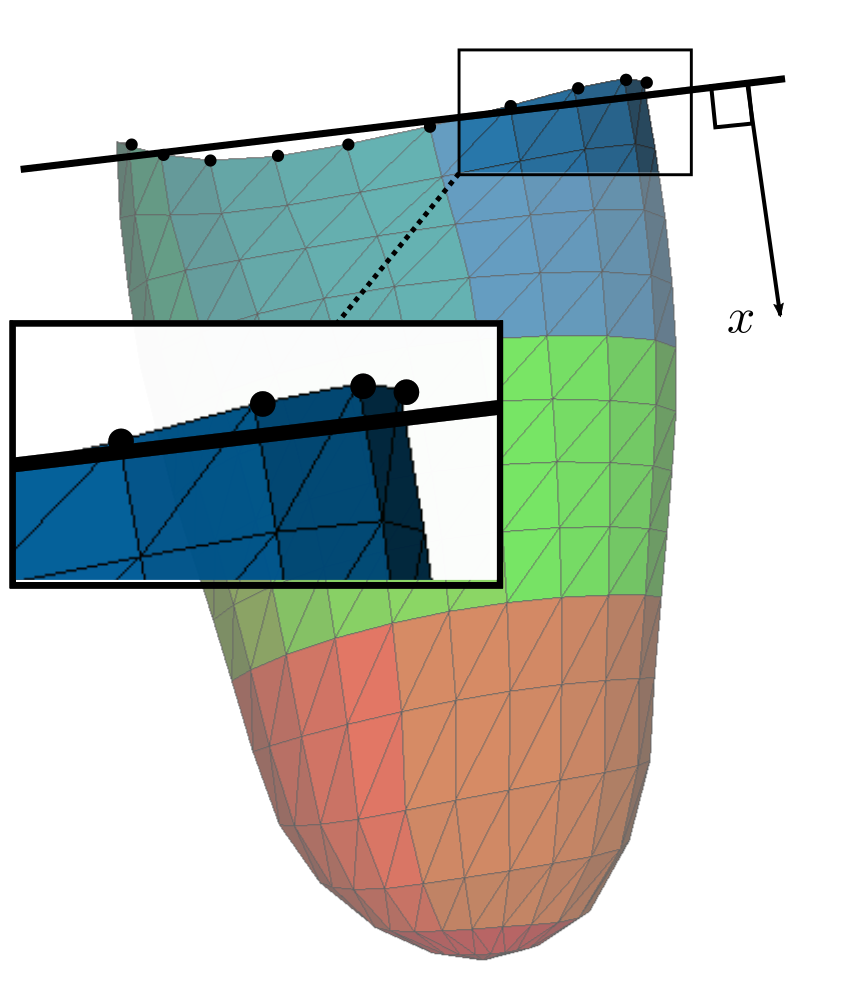
\includegraphics[width=\textwidth]{chapters/introduction/figures/geometry/strain_mesh_plane.pdf}
    \caption{\label{fig:strain_mesh_plane}}
  \end{subfigure}
  \begin{subfigure}[t]{0.45\textwidth}
    \includegraphics[width=\textwidth]{chapters/introduction/figures/geometry/cut.png}
    \caption{\label{fig:cut}}
  \end{subfigure}
\caption{}
\label{fig:echopac_output}
\end{figure}



The actualy mesh generation is performed using Gmsh
\cite{geuzaine2009gmsh}, which meshes the endocardial and epicardial
surface togther unsing frontal-Delaunay meshing algorithm. Gmsh also marks
the endocardal, the epicardial  and the basal facets, along with the
endocardial 

\begin{figure}[htbp]
  \centering
  \begin{subfigure}[t]{0.4\textwidth}
    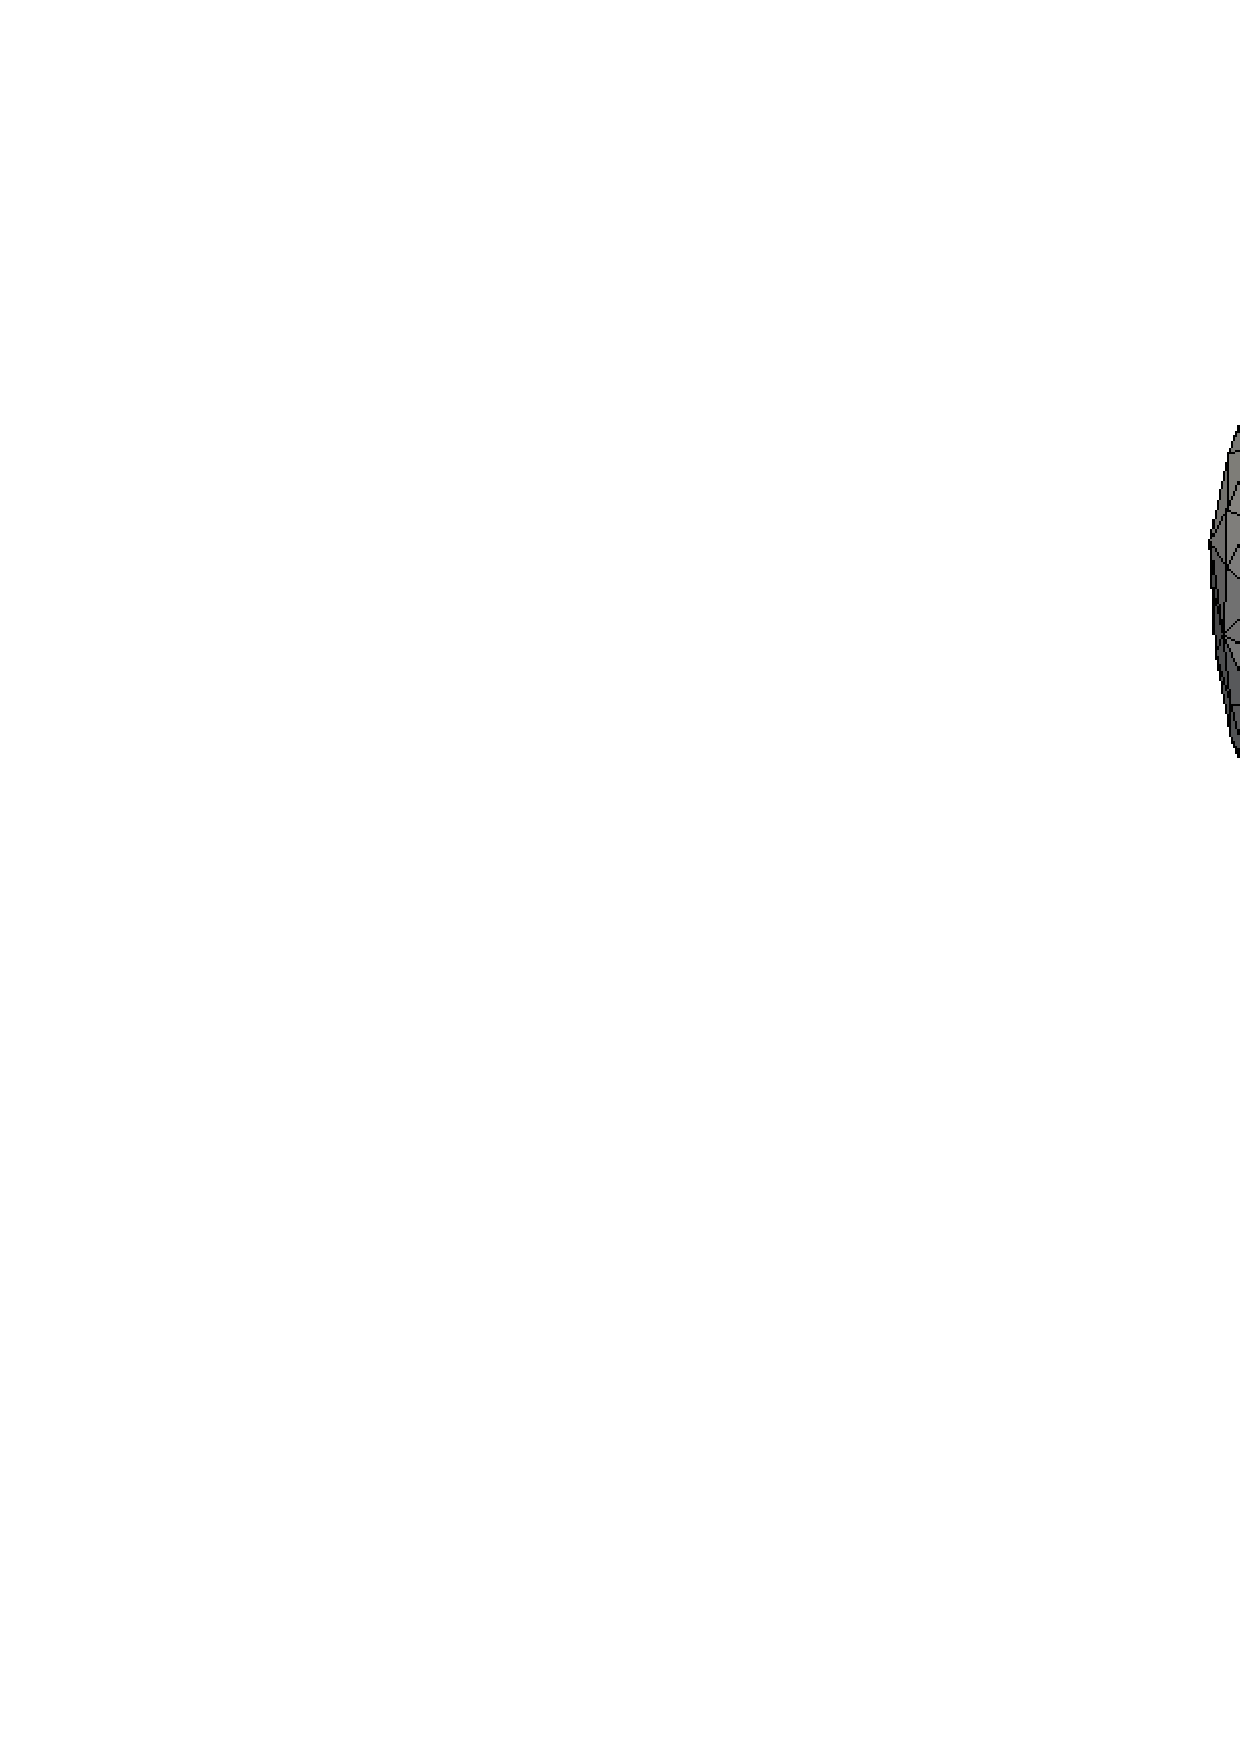
\includegraphics[width=\textwidth]{chapters/introduction/figures/geometry/mesh.png}
    \caption{\label{fig:mesh}}
  \end{subfigure}
  \begin{subfigure}[t]{0.45\textwidth}
    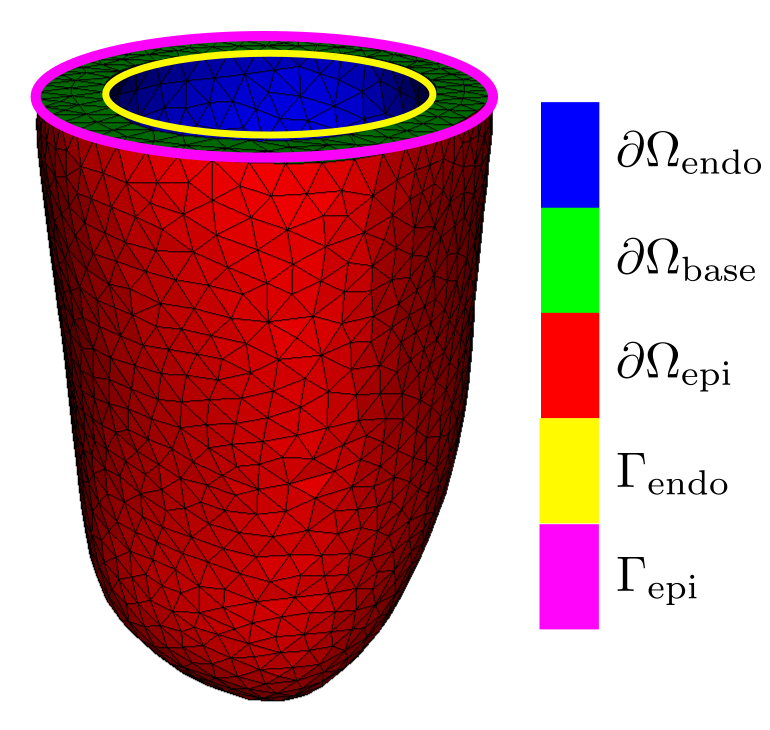
\includegraphics[width=\textwidth]{chapters/introduction/figures/geometry/markers_full.pdf}
    \caption{\label{fig:markers_full}}
  \end{subfigure}
\caption{}
\label{fig:echopac_output}
\end{figure}



\begin{remark}
  The cavity volume is computed by generating the whole mesh, and the
  compute the volume using Equation \eqref{eq:volume_operator}. The cut size is
  found by using a one dimensional optimization algorithm with
  the objective funcitonal representing the squared error between
  computed and measured volume.
\end{remark}




\subsubsection{Rule-based fibers}
\label{sec:rule_based_fiber}
Mention papers about fiber distribution, fiber dependence and
different rule-based fibers.

Describe the main steps in the Bayer algorithm. 


\subsubsection{The ventricular coordinate system}

When dealing with geometric shapes such as a left ventricle, finding a
coordinate system that is easy to work with is important. For
example, when studing spherical shapes, the spherical coordinate system is
usually easier to work with. Likewise, a coordinate system that is
easy to use when studying ellipsoidal shapes like the left ventricle is
the \emph{prolate spheroidal coordinate system} \cite{hunter1996kd}. 
The cartesian coordinates $(x,y,z)$ are related to the prolate
spheroidal coordinates by

\begin{align}
  \begin{split}
    x &= a \sinh \mu \sin \nu \cos \theta  \\
    y &= a \sinh \mu \sin \nu \sin \theta  \\
    z &= a \cosh \mu \cos \nu,
  \end{split}
\end{align}
where $a$ is the focal point, $\nu \in [0, \pi]$ is the longitudinal
coordinate, $\theta \in [0, 2\pi]$ is the azimuthal angle and $\mu$
is the radial coordinate. For an ellipse given by the equation
$\frac{x^2}{b^2} +\frac{y^2}{c^2}  = 1$ with $b$ being the semimajor
axis, and $c$ the semiminor axis, the focal point is given by
\begin{align}
  a =\sqrt{b^2 - c^2}.
  \label{eq:focal_point}
\end{align}
Assuming the ventricle is axisymetric around the
longitudinal axis, which is aligned with the $x$-axis it is possible
to estimate the focal point by taking $b$ in \eqref{eq:focal_point} to
be the maximum distance from the base to the apex, and $b$ the maximum
radius at the based. Using this estimate, the base is assumed to be
located approximately at the center of the ellipsoid, i.e $\nu = \pi /
2$. Compared to geometries used in benchmarking of cardiac mechanics
problems, this is not a totally wrong assumption
\cite{land2015verification}



\begin{figure}[htbp]
  \centering
  \begin{subfigure}[t]{0.4\textwidth}
    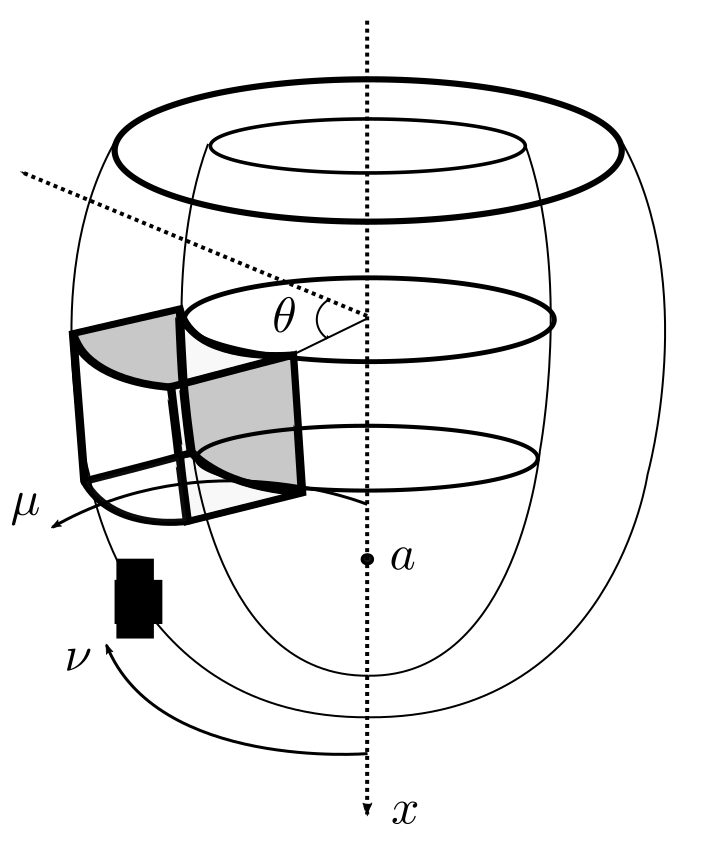
\includegraphics[width=\textwidth]{chapters/introduction/figures/geometry/prolate.png}
    \caption{\label{fig:prolate_coord}}
  \end{subfigure}
  \begin{subfigure}[t]{0.45\textwidth}
    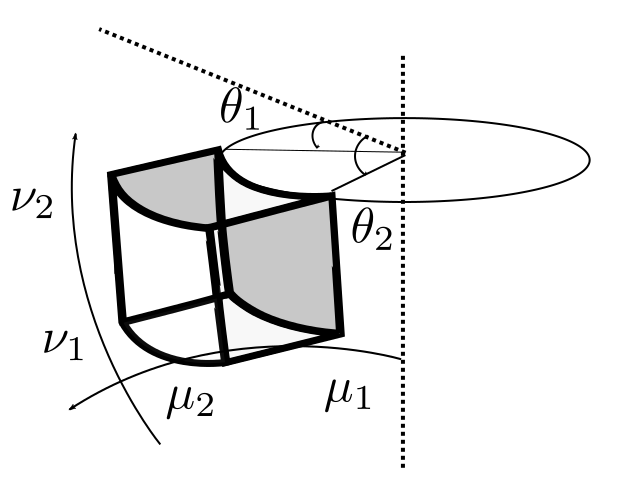
\includegraphics[width=\textwidth]{chapters/introduction/figures/geometry/prolate_cube.png}
    \caption{\label{fig:prolate_cube}}
  \end{subfigure}
\caption{}
\label{fig:prolate}
\end{figure}

\subsubsection{Marking the mesh according to the AHA-segments}



\begin{itemize}
  \item Segmentation and aquisition using echopach
  \item From closed endo- and epicardial surfaces to a mesh
    (smoothing, cutting, orienting).
  \item Marking of mesh accoring to AHA segments (16,17,18)
  \item Local basis
  \item Rule based fibers
  \item Referece to mesh{\_}generation and patient repositories
  \end{itemize}


\subsection{Data Assimilation}
The constitutive laws in cardiac mechanics comes from experiments
done on tissue slabs, and relates stresses in the material to strain.
If we had the same data available for a given patient we could easily
have performed a regression analysis in order to identify the
parameters in the contitutive model. However, this type of data
typically requires that tissue samples are taken from the myocardium,
which is not an option when dealing with living humans. In general,
when dealing with physical system such as the heart or weather
forecast it is not allways possible to design an experiment which
allows to determine all properties of a physical system
\cite{chapelle2013fundamental}. In such cases we have to take the
measurement that we have, and do our best to incorporate them into the
model. 

For example, the type of data that we usually have available, are data
that can be extracted using imaging techniques such as motion data,
volume traces, regional strain traces etc. One technique to estimate
model parameters based on such observations is called data assimilation.


The field of data assimilation has its roots in meteorology, where
a typical problem is to make predictions on the weather, based on
observations (of temperature, humidity etc.) at different locations. 


There are basically two main approaches to assimilate data;
\emph{sequential data assimilation} and \emph{variational data
  assimilation}. Sequential data assimilation, which is often
referred to as filtering, is based on a predictor-corector approach
where you start from your initial data and use a filter to predict the
next state. Once you have your measurement available you correct the
estimate based on the new observations. Some examples of sequential
procedures include Kalman filtering and Luenberger observers
\cite{chapelle2013fundamental}.

The other approach called variational data assimilation, which is the
one used in this thesis, is based on minimizing a cost functional that
represents the mismatch between observations and simulations, with
possibly additional regularization terms added to the objective
functional. 

% The general setup for a variational data assimilation problem is the
% following. 
We will now explain the general setup for variational data
assimilation. In order to keep consistent notation we will refer to
the \emph{state variable} as $\mathbf{w}$, which is our case
represents jointly the displacement and hydrostatic pressure
$\mathbf{w}=(\mathbf{u}, p)$.

The state varibles are described by some \emph{phyiscal
model} $\mathcal{L}$, which is our case is governed by the force balance
equations \eqref{eq:force_balance}, and can be written in the form
$\mathcal{L}\mathbf{w} = f$.

We are also given a set of measurements (or observations) that we want
to assimilate, and we denote this by the vector $\mathbf{y}$.
For example, $\mathbf{y}$ might be a set of volume measurements or a
combinations of volume and strain at given time points in the cardiac
cycle. The \emph{observation operator} $\mathcal{H}$, is approximation
of the observation and act as an operator from the state space to the
observation space. We therefore have the relation
\begin{align}
  \mathbf{y} = \mathcal{H}(\mathbf{w}) + \xi_o, 
\end{align}
where $\xi_o$ represents both the error in the measurements (e.g
noise in the data) and error in the representation of the observation
(that $\mathcal{H}$ do not represent the data good enough).


\paragraph{The volume observation operator
  $\mathcal{H}_{\mathrm{volume}}$}
In some cases, the ventricular cavity volume can easily be computed
analytically from the displacement field. Denote the inner cavity of
the left ventricle in the current configuration by
$\omega_{\mathrm{endo}}$. Further let $\mathrm{d} v$ and $\xvec$
denote an infinitesimal volume element and the coordinate in the
current configuration respectively. Then by the divergece theorem we have
\begin{align}
  \mathcal{H}_{\mathrm{volume}}(\uvec)= \int_{\omega_{\mathrm{endo}}} \mathrm{d} v =
  \frac{1}{3}\int_{\omega_{\mathrm{endo}}} \nabla \cdot \xvec \mathrm{d} v =
  \frac{1}{3}\int_{\partial \omega_{\mathrm{endo}}} \xvec \cdot \mathbf{n} \mathrm{d} s, 
\end{align}
where $\mathbf{n}$ and $\mathrm{d} s$ are the unit normal and a surface
element on the current configuration respectively.
Note that the boundary $\partial \omega_{\mathrm{endo}}$ includes the
endocardial basal boundary. However in the case when the base is flat
and fixed in longitudinal direction, the contribution from this
boundary integral will be zero. In this case the boundary integral
will be the same as the integral over the endocardial boundary
decribed in \ref{refer_to_section}, with the only change being the
change of sign on the normal vector. By Nansens formula we obtain
\begin{align}
  \mathcal{H}_{\mathrm{volume}}(\uvec)= -\frac{1}{3}\int_{\lvendo} \left( \Xvec + \uvec \right) J \F^{-T} \Nvec \mathrm{d}S,
  \label{eq:volume_operator}
\end{align}
where now $\lvendo$,  $\Xvec$, $\Nvec$ and $\mathrm{d}S$ are respectively the
endocardial surface, the referece coordinate, the unit normal and a
surface element in the reference configuration.


\paragraph{The strain observation operator
  $\mathcal{H}_{\mathrm{volume}}$}
Another observation that is encountered in this thesis is strain
measurements, of more precisely average regional strain in the
circumferential, radial or longitudinal direction. Let $\Omega_j$
denote the volume for which the strain should be averaged over, and
let $\mathbf{e}_k$ denote the unit vectorfield in the preferred strain
direction. Then for a given strain tensor $\mathbf{A}$ we define 
\begin{align}
  \mathcal{H}_{\mathrm{strain}}(\uvec) = \frac{1}{|\Omega_j|}\int_{\Omega_j} \mathbf{e}_k^T \mathbf{A}(\uvec) \mathbf{e}_k  \mathrm{d}V
\end{align}
The strain tensor $ \mathbf{A}$ is typically chosen to be the
Grenn-Lagrange strain tensor $\mathbf{E}$\eqref{eq:green_lagrange}, or
the material displacement gradient tensor $\F - \I$.

\begin{remark}
  Measured strains are computed relative to some reference
  geometry, which do not always coinside with the reference geometry
  chosen for your simulation. In these cases you have to either
  recompute the measured strain according to the chosen referece for
  the simulation, or recompute the simulated strains according to the
  correct referece geometry for your measuments. 
\end{remark}

% Within varitaional data assimilation it is common to separate between
% dynamic models and static models. These are conventionally reffered to as
% $4D-$Var and $3D-$Var methods respectively. In the work done this
% thesis we have used both of these methods. 


% For an introduction to data assimilation we refer to e.g \cite{lahoz2010data}.

Let us assume that 


\begin{itemize}
  \item Examples of data you want to constrain
  \item Forming of mismatch functional and problem formulation as
    PDE-constrained optimization.
  \item The adjoint approach. comparison with other methods.
  \item Control parameters
  \item OPtimization algorithm - stopping criteria
  \item Reference to pulse{\_}adjoint and pulse{\_}adjoint{\_}post
    repositories
  \item Variational versus sequnetial
  \item Question about uniquness
\end{itemize}


We will now explain what we mean by ``adjoint-based'', and why this
approach is a key ingredient. The main theory presented here is taken
from the dolfin-adjoint web page. A word about dolfin adjoint...\ref{}
  
\begin{equation}
  \begin{aligned}
    \label{eq:opt_matparam}
    & \underset{\mvec}{\text{minimize}}
    & &  \mathcal{J}(\state, \mvec) \\
    & \text{subject to}
    & & \delta \Pi(\state, \mvec) = 0, 
  \end{aligned}
\end{equation}

where $\mathcal{J}(\state, \mvec): \mathbb{W} \times \mathbb{Q} \mapsto
\mathbb{R}$ for some state space $\mathbb{W}$ and parameter space
$\mathbb{Q}$ and $\delta \Pi(\state, \mvec)) = 0$ is the force balance
equation given by \ref{}.
$\mvec = (m_1, \cdots m_P)$


Now suppose we have discretized the partial differental equation
$\delta \Pi(\state, \mvec) = 0$, which reduces to a system of the form
$\mathbf{A} \state = \mathbf{b}$, with possible all terms depending on
the parameters $\mvec$. The gradient of the cost functional with
respect to the parameter is given by
\begin{align}
  \frac{\mathrm{d} \mathcal{J}}{\mathrm{d} \mvec} = \frac{\partial \mathcal{J}}{\partial \mvec}
  + \frac{\partial \mathcal{J}}{\partial \state} \frac{\mathrm{d} \state}{\mathrm{d} \mvec}.
  \label{eq:grad_cost}
\end{align}
Here $\frac{\mathrm{d}}{\mathrm{d} \mvec}$ denotes the total
derivative, while $ \frac{\partial}{\partial \mvec}$ denotes the
partial derivative. Computing the partial derivatives in
\eqref{eq:grad_cost} are usually straight forward, while computing  $
\frac{\mathrm{d} \state}{\mathrm{d} \mvec}$ is hard. To see this, let
us differentiate the equation $\mathbf{A} \state = \mathbf{b}$ with
respect to $m_i$, and solve for the 


\begin{remark}
  In data assimilation we typically want to copmute the gradient of
  the cost function because we want to employ gradient-based
  optimization algorithms for finding the ``optimal'' parameter
  set. In other cases, the gradient might be important because it
  tells you something about the sensitivity of your function of
  interest with respect to the parameters. For example, if you have a
  model with many input parameters, you may want to identify what
  impact the different parameters has on the output. Perturbing each
  parameter and observing the chane in the objective function quickly
  becomes infeasible when the number of parameters becomes large, in
  which case the adjoint aproach offer a possible solution. 
\end{remark}



\subsubsection{Adjoint method}
In order to apply optimisation algorithm...
We reduce the objective functional to be a function of the control
parameters only, $\hat{I}(\mvec) := I(\state(\mvec), \mvec)$. Consider an
initial value of the parmameters $\mvec = \mvec^0$. If $\hat{I}(m)$ is defined
and differentible in a neighborhood of $\mvec^0$ then $\hat{I}$ (and
consequently $I$) decreases fastest in the direction of the gradient, 
\begin{align}
  \nabla_{\mvec} \hat{I}(\mvec^0) = \begin{bmatrix}
    \frac{\mathrm{d} \hat{I}(\mvec^0) }{\mathrm{d} m_1},
    \frac{\mathrm{d} \hat{I}(\mvec^0) }{\mathrm{d} m_2},
    \cdots
    \frac{\mathrm{d} \hat{I}(\mvec^0) }{\mathrm{d} m_N}
  \end{bmatrix}^T.
  \label{eq:functional_gradient}
\end{align}
Here $\frac{\mathrm{d} \hat{I} }{\mathrm{d} m_i}$ represents the
total derivative:
\begin{align}
  \frac{\mathrm{d} \hat{I} }{\mathrm{d} m_i} = \frac{\mathrm{d} I (\state(\mvec), \mvec))}{\mathrm{d} m_i} = \frac{\partial  I }{\partial \state} \frac{\mathrm{d} \state}{\mathrm{d} m_i} + \frac{\partial  I }{\partial m_i}.
  \label{eq:functional_derivative_component}
\end{align}
In other words, the sequence
\begin{align}
  \mvec^{k+1} = \mvec^{k} - \gamma_k \nabla_{\mvec} \hat{I}(\mvec^k), \gamma_n \in \mathbb{R}
\end{align}
satisfies $\hat{I}(\mvec^{k+1}) \leq \hat{I}(\mvec^k) \; \forall k \geq
0$, and converges towards a local minimum. If $\hat{I}$ is convex then
the minimum is also global.
Being able to compute the gradient of the objective functional wrt to
the control parameters allows us to employ gradient based optimization
methods which are in general superior to gradient free methods.
One way to compute the gradient is by means of the finite difference
approach: For a given parameter $\mvec = \mvec^*$ we have
\begin{align}
  \frac{\mathrm{d} \hat{I} }{\mathrm{d} m_i}( \mvec^*) =
  \lim_{h \mapsto 0} \frac{\hat{I}(\mvec^* + h\mathbf{e}_i) - \hat{I}(\mvec^*)}{h}, 
\end{align}
where $\mathbf{e}_i \in \mathbb{Q}$ is the $i$'th canonical basis
vector. If $\dim(\mathbb{Q}) = N$, this approach would require $N+1$
functional evaluations. Moreover, since the state-variables depends upon the
control variables, we would also need to solve the force balance
equation $N+1$ times, which is typically very copmutationally
expensive. Hence, this approach is typically infeasable when the
dimesion of your parameterspace is large. In this case the adjoint
approach is much better. If $A$ is an operator (e.g a matrix), then
the adjoint operator $B$ satisfies the relation $\langle Au, v \rangle
= \langle u, Bv \rangle$, and we write $ B = A^*$. Here $(\cdot)^*$
denotes the Hermitian transpose, which in the case where $A$ is a real
matrix is just the transpose of $A$, $A^T$.  


Note that the gradient in
\eqref{eq:functional_gradient} can be rewritten (using the chain rule)
as
\begin{align}
  \nabla_{\mvec} \hat{I} =  \frac{\partial  I }{\partial \state} \nabla_{\mvec} \state
  + \frac{\partial  I }{\partial \mvec},
  \label{eq:functional_gradient_chain}
\end{align}
in which the $\dim(\mathbb{V}) \times \dim(\mathbb{Q})$ matrix
$\nabla_{\mvec} \state$ is difficult to compute.
Differentiating the force-balance equation \ref{} with respect to the
control parameters yields
\begin{align}
  & \nabla_{\mvec} \delta \Pi(\state, \mvec) = 0 \\
  \implies & \frac{\partial  \Pi }{\partial \state} \nabla_{\mvec} \state
  + \frac{\partial  \Pi }{\partial \mvec} = 0 \\
  \implies & \nabla_{\mvec} \state =
             - \left( \frac{\partial  \Pi }{\partial \state} \right)^{-1} \frac{\partial  \Pi }{\partial \mvec}.
\end{align}
Inserting this expression for $\nabla_{\mvec} \state$ into
\eqref{eq:functional_gradient_chain}, gives
\begin{align}
  \nabla_{\mvec} \hat{I} =  - \frac{\partial  I }{\partial \state}
  \left( \frac{\partial  \Pi }{\partial \state} \right)^{-1} \frac{\partial  \Pi }{\partial \mvec}
  + \frac{\partial  I }{\partial \mvec}.
\end{align}


\subsubsection{Dolfin-Adjoint}

Dolfin-Adjoint is a software package that based on the FEniCS project
which aims to derrive the discrete adjoint equation and the tangent
linear models of finite element models implemented within the FEniCS
framework. While the tradional approach is to derrive the adjoint code
from the forward code using automatic differentiation tools,
Dolfin-Adjoint utilises the high level symbolic representation
\cite{UFL} in FEniCS to derrive the discrete adjoint equations from
the discrete forward eqations, and then the FEniCS system derrives the
adjoint code from the discrete adjoint equations. 

\subsubsection{Optimization methods}

Line search methods, interior point methods, gradient based methods,
genetic methods, trust region



\subsection{Identifiability of parameters}
% Try dividing heart mesh is different segment, discuss uniqueness of
% paraperers
% Discuss regularization technices
When dealing with parameter estimation, you should always consider
questions about identifiability and uniquness. This depends on the
model, the data and the objective functional
\cite{hadjicharalambous2015analysis}. A first test should be to
generate synthetic data with some prescribed parameters, feed this
error-free data to the data assimilation method, and ensure that you
are able to retrieve the parameters that generated that data. If you
end up with a different parameter set than the one generated the data,
your problem is not \emph{structuraly identifiable}
\cite{chabiniok2016multiphysics}. Your problem is said to be
\emph{practical identifiable} if the parameters can be determined
uniquely based on the data at hand. If the test passes you shold try
to add noise to the data, and see if your data assimilation is stable
with respect to noise in the measurement, and you should quantify the
model out error versus the model input error. Demonstrating identifiability is
often difficult, especially when your data is corrupted with noise,
and when the complexity of the model increases. Balancing the
complexity of model in terms of \emph{model fidelity}, i.e wheter your
model is rich enough to representing the data, and the identifiability
is often key in order to have robust model. A too simple model will
often fail to represent your data, while a too complex model, might
give completely differet answers with just a slight perturbation of
the data, i.e with noise added to the measurement. The same problem is
encountered in other scientific disiplines, for instance in
statistical learning theory, \emph{overfitting} is related to
overparameterization of the model, in which you can perfectly
represent your data, but a small perturbation will cause a significant
error. Another problem, which is also related to identifiability is
the question about uniquness of the soluton. A practical test is to
start the optimization algorithm from different intial points and see
if you end up at the same optimum. If this does not happen, it is
likely that the objective functional is not convex, which is a
requirement for uniquness. Unfortunately, this is the case for many
problems in PDE-constrained optimization. In these cases, the objective
functional might have several distinct local minima, in which case
different techniques for find the best local minima exists
\cite{farrell2015multiple}. 

\subsubsection{An example of a non-structuraly identifiable problem}
Split the ventricle in two, and use volume as the only input.
Show that differnt parameter sets (with $\gamma$) will generate the
same volume



\subsubsection{Material parameter estimation}

\paragraph{One volume measurement only}

\paragraph{Multiple volume measurements}

\paragraph{Volume and strain measurements}

\subsubsection{Coupled unloading and material parameter estimation}
In Section \ref{sef:reference_geometry} we described a method for
finding the uloaded configuration unsing the backward displacement
method. The problem of using this method when dealing with parameter
estimation is that the unloaded geometry depends on the material
properties, which in general is unknown. Hence we need a way of
estimating both the unloaded geometry and the material parameters at
the same time. One possibible algorithm is the following:



\begin{algorithm}
\caption{Coupled Unloading and material parameters estimation}\label{alg:unloaded_material}
\begin{algorithmic}[1]
  \State $i = 0$
  \State residual = $\infty$
  \State $\mvec_0 =  \mvec$ \Comment{Initial guess for material parameters}
  \While{i $<$ N and residual > tolerance }

  \State $\Omega_{\mathcal{U}}^i$ = Unload($\Omega_{\mathcal{I}}, \mvec_i$) \Comment{unload
    material}
  \State $\mvec_{i+1}$ = EstimateMaterial($\Omega_{\mathcal{U}}^i,
  \mvec_i$) \Comment{estimate material parameters}
  \State residual = ComputeResidual($\Omega_{\mathcal{U}}^i,
  \Omega_{\mathcal{U}}^{i-1}$)
  \State $i = i +1$
 
  \EndWhile
\end{algorithmic}
\end{algorithm}

\subsection{Activation parameter estimation}



\subsubsection{Multiobjetive optimization}
Paramaters in the model are estimated based on minimizing a cost
functional representing the mismatch between observations and simulaton.
Assume we are given $N$ different observations, then in priciple we
have $N$ different cost funcitonals to solve
\begin{equation}
  \begin{aligned}
    \label{eq:multiobjetive_opt}
    & \text{minimize}
    & &  \left\{ \mathcal{J}_1(\lambda), \mathcal{J}_2(\lambda), \cdots, \mathcal{J}_N(\lambda) \right\} \\
    & \text{subject to}
    & & \delta \Pi(\state(\lambda)) = 0, \lambda \in \mathcal{P},
  \end{aligned}
\end{equation}
whith 
\begin{align}
  \mathcal{J}_i(\lambda) = \left( \mathbf{y} - \mathcal{H}(\state(\lambda)) \right)^2, \; i = 1,\cdots, N
\end{align}
The above observations comes from the same soure, and hence it should
be intuitive that minimizing one of them, would also bring the other
closer to a minimum. However, with precense of noise in the data,
this might not always be the case, and hence we have a conflicting
objectives. Problem \eqref{eq:multiobjetive_opt} is called a
multiobjetive optimization problem \cite{deb2016multi}. Such problems
typically do not have a single optimal solution, but a family of
solutions called \emph{Pareto optmal solutions}. The basic methods for
solving such problems inclues \emph{the weighted method}, \emph{the
  $\varepsilon$-constraint method}, 




\subsection{Mehcanical biomarkers}
A word about what models can contribute with




%%% Local Variables:
%%% mode: latex
%%% TeX-master: "../../main"
%%% End:
